\documentclass[tikz,border=8pt]{standalone}
\usepackage{amsmath}
\usepackage{pgfplots}
\pgfplotsset{compat=1.18}
\usetikzlibrary{arrows.meta,calc,decorations.pathmorphing}
\definecolor{ink}{HTML}{17324D}
\definecolor{blue}{HTML}{1877B8}
\definecolor{orange}{HTML}{D97706}
\definecolor{green}{HTML}{16856B}
\definecolor{red}{HTML}{C24156}
\begin{document}
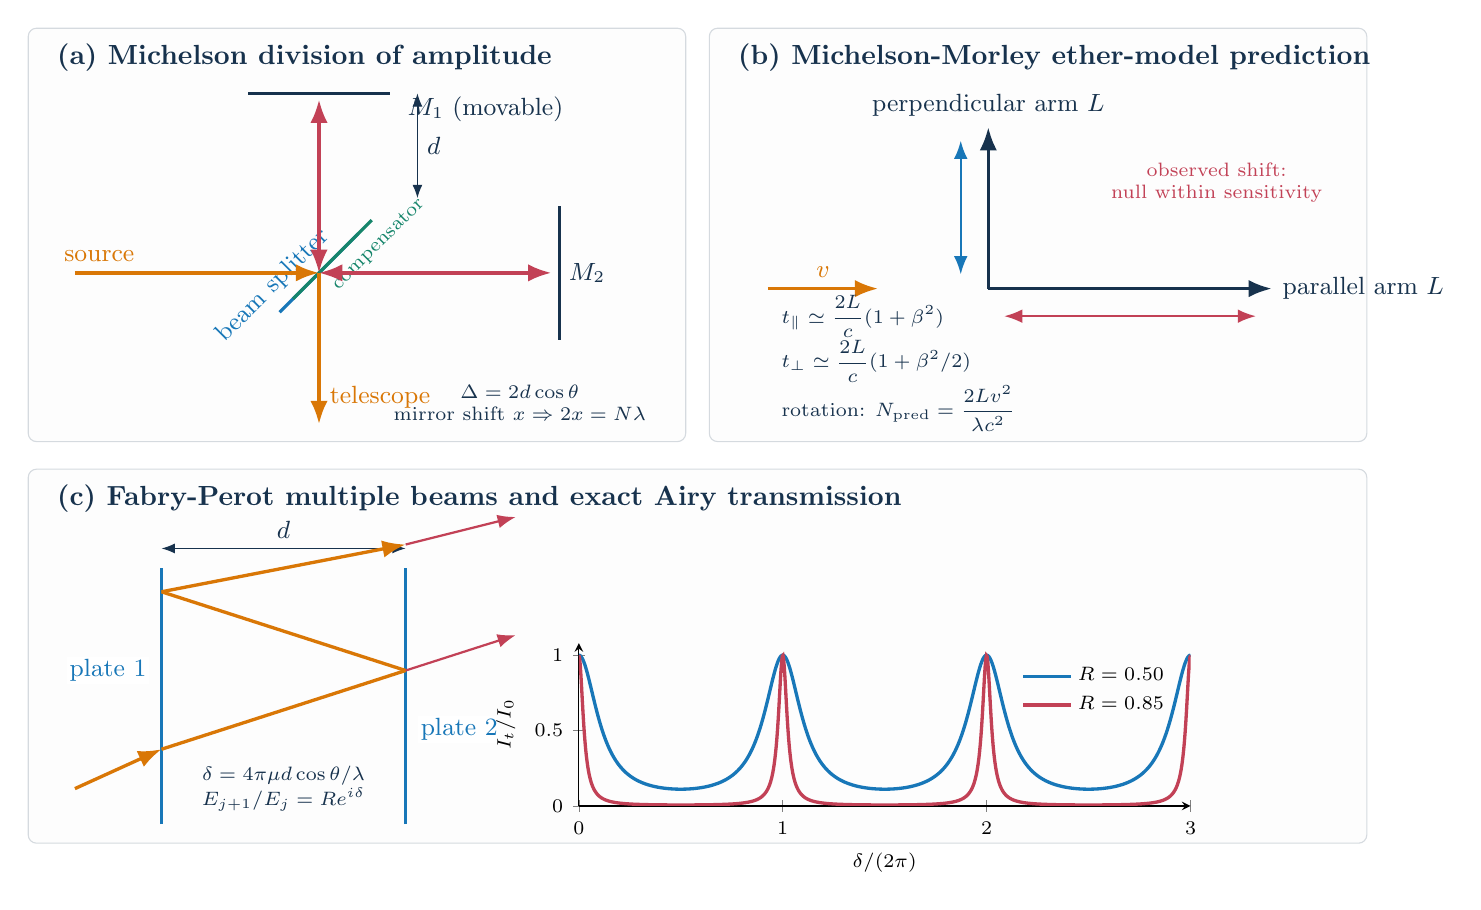
\begin{tikzpicture}[font=\small,>=Latex]
\tikzset{panel/.style={draw=ink!18,rounded corners=3pt,fill=ink!1}}

\node[panel,minimum width=8.35cm,minimum height=5.25cm,anchor=south west] at (0,5.1) {};
\node[font=\bfseries,ink,anchor=west] at (.25,9.98) {(a) Michelson division of amplitude};
\begin{scope}[shift={(.55,5.15)}]
  \coordinate (B) at (3.15,2.10);
  \draw[very thick,blue] (2.65,1.60)--(3.65,2.60);
  \node[blue,rotate=45,anchor=south] at (2.75,1.75) {beam splitter};
  \draw[very thick,green] (2.82,1.77)--(3.82,2.77);
  \node[green,rotate=45,font=\scriptsize,anchor=north] at (3.75,2.62) {compensator};
  \draw[very thick,ink] (2.25,4.38)--(4.05,4.38);
  \node[ink,anchor=west] at (4.15,4.18) {$M_1$ (movable)};
  \draw[very thick,ink] (6.20,1.25)--(6.20,2.95);
  \node[ink,right] at (6.20,2.10) {$M_2$};
  \draw[->,orange,very thick] (.05,2.10)--(B) node[pos=.1,above] {source};
  \draw[<->,red,very thick] (B)--(3.15,4.30);
  \draw[<->,red,very thick] (B)--(6.10,2.10);
  \draw[->,orange,very thick] (B)--(3.15,.18) node[pos=.82,right] {telescope};
  \draw[<->,ink] (4.40,3.05)--(4.40,4.38) node[midway,right] {$d$};
  \node[align=center,font=\scriptsize,ink] at (5.70,.45)
    {$\Delta=2d\cos\theta$\\mirror shift $x\Rightarrow2x=N\lambda$};
\end{scope}

\node[panel,minimum width=8.35cm,minimum height=5.25cm,anchor=south west] at (8.65,5.1) {};
\node[font=\bfseries,ink,anchor=west] at (8.90,9.98) {(b) Michelson-Morley ether-model prediction};
\begin{scope}[shift={(9.25,5.05)}]
  \coordinate (O) at (2.95,2.0);
  \draw[->,ink,very thick] (O)--(6.55,2.0) node[right] {parallel arm $L$};
  \draw[->,ink,very thick] (O)--(2.95,4.05) node[above] {perpendicular arm $L$};
  \draw[<->,red,thick] (3.15,1.65)--(6.35,1.65);
  \draw[<->,blue,thick] (2.60,2.18)--(2.60,3.88);
  \draw[->,orange,very thick] (.15,2.0)--(1.55,2.0) node[midway,above] {$v$};
  \node[align=left,font=\scriptsize,ink,anchor=west] at (.20,1.05)
    {$t_\parallel\simeq\dfrac{2L}{c}(1+\beta^2)$\\
     $t_\perp\simeq\dfrac{2L}{c}(1+\beta^2/2)$\\
     rotation: $N_{\rm pred}=\dfrac{2Lv^2}{\lambda c^2}$};
  \node[red,font=\scriptsize,align=center] at (5.85,3.35)
    {observed shift:\\null within sensitivity};
\end{scope}

\node[panel,minimum width=17cm,minimum height=4.75cm,anchor=south west] at (0,0) {};
\node[font=\bfseries,ink,anchor=west] at (.25,4.38) {(c) Fabry-Perot multiple beams and exact Airy transmission};
\begin{scope}[shift={(.55,.15)}]
  \draw[very thick,blue] (1.15,.10)--(1.15,3.35);
  \draw[very thick,blue] (4.25,.10)--(4.25,3.35);
  \node[blue,anchor=east,fill=white,inner sep=1pt] at (1.00,2.05) {plate 1};
  \node[blue,anchor=west,fill=white,inner sep=1pt] at (4.40,1.30) {plate 2};
  \draw[<->,ink] (1.15,3.60)--(4.25,3.60) node[midway,above] {$d$};
  \draw[->,orange,very thick] (.05,.55)--(1.15,1.05);
  \draw[orange,very thick] (1.15,1.05)--(4.25,2.05);
  \draw[orange,very thick] (4.25,2.05)--(1.15,3.05);
  \draw[->,orange,very thick] (1.15,3.05)--(4.25,3.65);
  \draw[->,red,thick] (4.25,2.05)--(5.65,2.50);
  \draw[->,red,thick] (4.25,3.65)--(5.65,4.00);
  \node[align=center,font=\scriptsize,ink] at (2.70,.55)
    {$\delta=4\pi\mu d\cos\theta/\lambda$\\$E_{j+1}/E_j=Re^{i\delta}$};
\end{scope}
\begin{axis}[at={(7.0cm,.48cm)},anchor=south west,width=9.35cm,height=3.65cm,
  axis lines=left,xlabel={$\delta/(2\pi)$},ylabel={$I_t/I_0$},xmin=0,xmax=3,ymin=0,ymax=1.08,
  xtick={0,1,2,3},ytick={0,.5,1},tick label style={font=\scriptsize},label style={font=\scriptsize},
  legend style={font=\scriptsize,draw=none,fill=none,at={(.98,.92)},anchor=north east}]
  \addplot[blue,very thick,domain=0:3,samples=700]{1/(1+(4*.50/(1-.50)^2)*sin(deg(pi*x))^2)};
  \addlegendentry{$R=0.50$}
  \addplot[red,very thick,domain=0:3,samples=900]{1/(1+(4*.85/(1-.85)^2)*sin(deg(pi*x))^2)};
  \addlegendentry{$R=0.85$}
\end{axis}
\end{tikzpicture}
\end{document}
